\chapter[Desenvolvimento]{Desenvolvimento}


A \autoref{diagrama} apresenta a topologia básica do projeto abordado neste trabalho por meio de um diagrama de blocos. 
O conjunto é composto por um microcontrolador \texttt{Arduino DUE} responsável pela aquisição dos eventos gerados pelos sensores.
Na seção \ref{due} são apresentados mais detalhes a respeito desse microcontrolador. O bloco de sensores é constituído em primeiro memento 
por um conjunto de seis sensores magnéticos que serão instalados nos portões. Esse tipo de sensor é bastante utilizado nesse tipo de aplicação
(detecção de abertura/fechamento de portões, portas e janelas). Seu funcionamento se dá de maneira bem simples, a partir de um campo magnético 
geralmente proveniente de um imã permanente ou de uma bobina. Tem o mesmo princípio de funcionamento de um gerador elétrico. A interface \texttt{Web} é 
composta por um módulo \texttt{ethernet R3}, seu \texttt{chip Wiznet W5100} fornece uma rede \texttt{IP} compatível com os protocolos \texttt{TCP} e \texttt{UDP}. Conforme apresenta a sua
documentação, esse \texttt{chip} tem como caraterística a sua facilidade de integração, programação e grande estabilidade. A central \texttt{IHC} local será composta
por um display \texttt{LCD} que exibirá algumas informações úteis em tempo real relacionadas ao status do sistema. Os eventos detectados e tratados pelo
microcontrolador compõem a base de dados do servidor.  A partir desses dados uma interface \texttt{IHC} remota os apresentará de maneira amigável ao operador
do sistema. 

\begin{figure}[h]
	\centering
	\caption{\label{diagrama}Topologia do projeto.}
		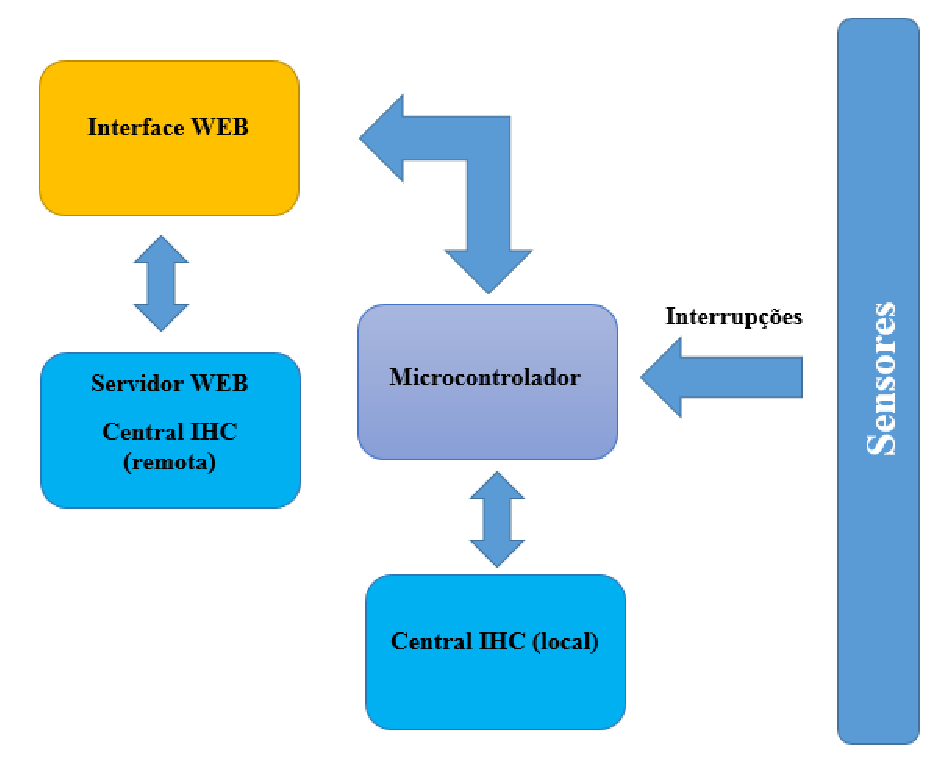
\includegraphics[keepaspectratio=true,scale=0.7]{figuras/diagrama.eps}
	\fonte{Autoria própria.} % Referencia errada
\end{figure}


\section{\textit{Arduino DUE}}



O microcontrolador escolhido para compor a central de aquisição de dados é o \texttt{Arduino DUE}, equipado com um \texttt{chip} de 32 \textit{bits} \texttt{ARM Cortex-M3}, 
mais precisamente o modelo \texttt{Atmel SAM3X8E} fabricado pela própria \texttt{Atmel}. A escolha dessa plataforma pode ser 
justificada devido ao seu baixo custo de aquisição, alto poder de processamento e facilidade de configuração. Foi o microcontrolador que 
apresentou a melhor relação custo x benefício dentre os analisados (modelos da família \texttt{PIC} e alguns modelos fabricados pela \texttt{Freescale}). 
O seu núcleo permite que operações de 4 \textit{bytes} sejam realizadas em um único clico de \textit{clock}. A frequência de operação nativa é de 84 \textit{MHz}. 
Entre as suas demais especificações, estão uma memória \textit{flash} de 512 \textit{KB} e 96 \textit{KB} de \texttt{SRAM} que garante muito mais recursos para programas 
maiores e mais complexos. A \autoref{due} apresenta uma visão da frente e do verso da placa.

\begin{figure}[h]
	\centering
	\caption{\label{due}\texttt{Arduino DUE}.}
		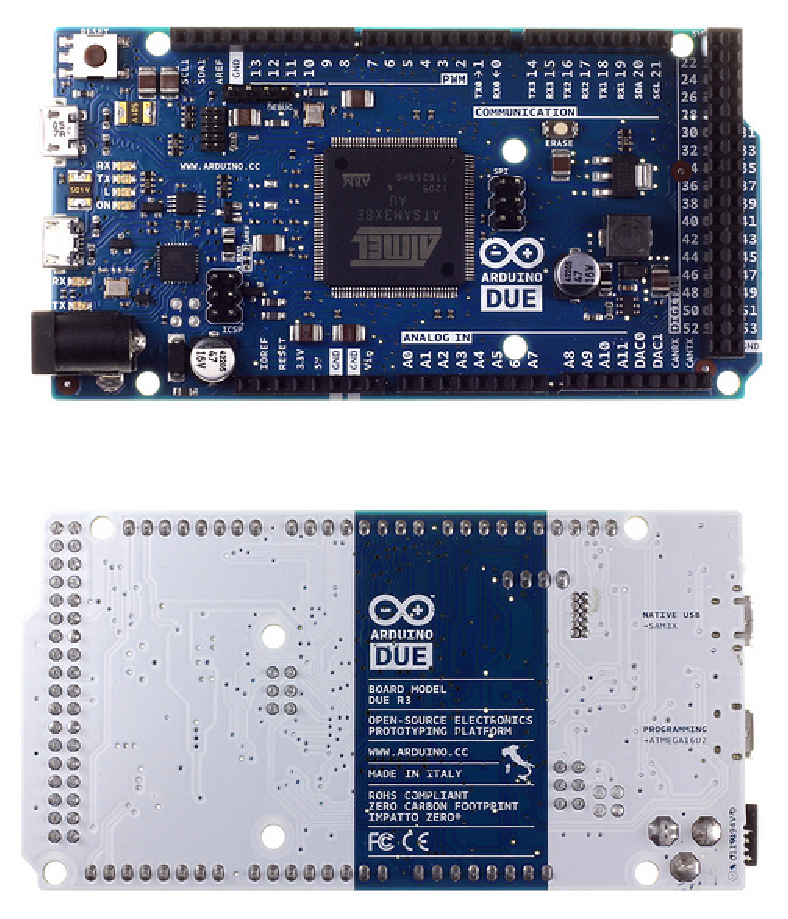
\includegraphics[keepaspectratio=true,scale=0.7]{figuras/due1.eps}
	\fonte{\cite{dueref}.} % Referencia errada
\end{figure}


A placa possui um total de 54 pinos digitais de \texttt{I/O}, em que desses, 12 podem ser utilizados como controle \texttt{PWM}. O seu conversor 
\texttt{ADC} é incrivelmente rápido podendo operar em uma frequência de amostragem de até 1 \textit{MHz} com 12 \textit{bits} de resolução. Além disso, possui 
dois conversores \texttt{DAC} também de 12 \textit{bits} de resolução. Possui 54 pinos digitais de entrada e saída. A tensão de operação dos pinos é de 3,3 V. 
Porém, uma das característica que mais despertou atenção nesta placa é a possibilidade de configurar praticamente todos os seus pinos para 
trabalharem com interrupções de \textit{hardware}. Devido a sua robustez, o \texttt{Arduino DUE} é bastante utilizando em tarefas de captura e processamento de 
áudio ou no controle de vários motores.

